\section{Reweighting the model's own samples fails}
\label{sec:exp-validity}
On the eleven pools we drew $S=16$ reasonings per training question under the incumbent
($\tau=0.7$, no top-$k$/top-$p$ truncation) and computed exact tempered likelihood ratios under
every candidate (Appendix~\ref{app:dist}). The primary predictor, registered for hypothesis
H-dist, is Eq.~\ref{eq:snis} with candidate reads at the label-free $\beta^\ast$ ($\tfrac12$ in
eight pools, $\tfrac14$ in two, $1$ in one). Its kill criterion was fixed before any of this data
existed (Appendix~\ref{app:prereg}): beat a random shortlist in pooled best-3 regret (paired
bootstrap $P(\text{gain}>0)\ge0.9$, and in at least $7$ of $11$ pools), and fall no more than $0.05$
below fresh greedy accuracy on $8$ questions (fresh-8) in pooled Spearman. H-inc applies it to the
distribution term alone (incumbent reads); defined after the first pool, it is confirmatory on the
other ten.

\paragraph{Both registered hypotheses fail all three conditions.} The primary predictor has a
pooled Spearman of $+0.034$ (bias-corrected interval $[-0.065,+0.190]$, conditional on the pools).
Its best-3 regret, $0.075$, is higher than the random shortlist's $0.067$ (gain $-0.009$
$[-0.027,+0.008]$, $P(\text{gain}>0)=0.21$; lower regret in $6$ of $11$ pools), and its Spearman is
$0.243$ below fresh-8. On pools 2--11, H-inc has pooled Spearman $-0.024$, regret $0.083$ against
$0.069$ for random ($6$ of $10$ pools, $P=0.18$) and a Spearman $0.280$ below fresh-8. H-dist and
H-inc are not supported (Table~\ref{tab:hdist}, Appendix~\ref{app:dist}).

\paragraph{No tempering recovers a signal, and the score is noise.} Across
$\beta\in\{0,\tfrac14,\tfrac12,1\}$ all estimates (candidate, incumbent or soft reads) have pooled
Spearman $-0.016$ to $+0.060$, every bias-corrected interval containing zero
(Figure~\ref{fig:beta}); with soft reads at $\beta=0$, the objective's sampled analogue is null
($-0.016$), against $-0.258$ on greedy reasoning. Regret falls toward $\beta=1$ ($0.056$--$0.062$)
without a rank signal, and the first-order score function is worse than random (regret $0.089$).
The primary score's split-half reliability is $-0.31$ to $+0.26$ per pool (a diagnostic added after
five pools, like a KL gate that stays below fresh-8; Table~\ref{tab:hdist}, Appendix~\ref{app:dist}).

\begin{figure}[t]
\centering
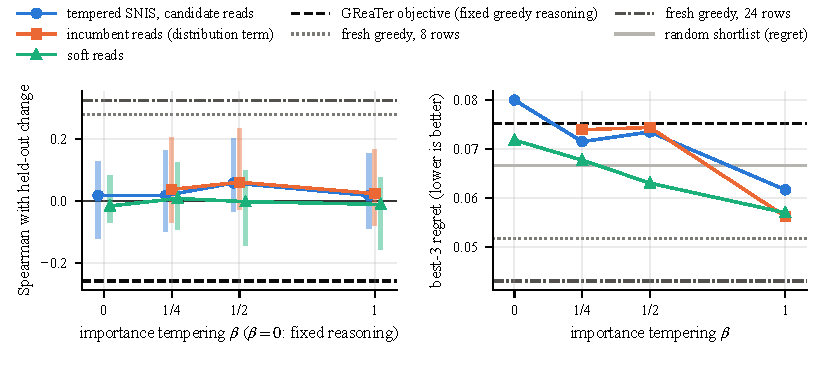
\includegraphics[width=0.85\linewidth]{figures/beta.pdf}
\caption{\textbf{Reweighting the incumbent's samples does not recover a ranking signal at any
tempering} (registered H-dist test, 11 pools; $\beta=0$: no reweighting). Left: pooled Spearman with
the held-out change for SNIS with candidate, incumbent (distribution term only) and soft reads;
bars: bias-corrected bootstrap ranges. Lines: the fixed-reasoning objective on the greedy reasoning
(\greater{} objective) and fresh greedy accuracy on $8$ and $24$ training questions (rows). Right:
best-3 regret (lower is better); random shortlist $0.067$.}
\label{fig:beta}
\end{figure}

\section{Verification budget decides}
\label{sec:exp-verify}
What an edit does must therefore be observed on fresh reasoning, a noisy instrument even under a
deterministic engine: if the fraction $f$ of questions whose correctness flips between two prompts
carries no systematic sign, their accuracy difference on $n$ questions has variance $f/n$, a
standard deviation of about $14$--$16$ points on $8$ questions and $3$ on $200$ at the flip rates of
single-token edits (Appendix~\ref{app:noise}). These analyses are exploratory; the matched-cost and
fixed-budget replays were specified after the registered outcome, the pipeline simulation of
Appendix~\ref{app:pipeline} before it. An edit is scored by its mean correctness change over the
incumbent on $G$ generations per candidate, greedy ($G$ questions) or sampled ($k$ samples at
$\tau=0.7$ on each of $r$ questions, $G=rk$; incumbent on the same seeds or on independent ones),
averaged over $400$ random subsets (Figure~\ref{fig:verify}).

\paragraph{Quality rises with generations, not with sampling or coupling.} Pooled Spearman rises
monotonically with $G$ for every verifier, from $+0.178$ for $4$ greedy reads to $+0.325$ for $24$
and $+0.413$ for $24\times4$ samples. At equal $G$, sampled reads rank worse than greedy ones in all
$15$ matched comparisons (by $0.03$--$0.06$, none significant alone), and common random numbers
\citep{corvelobenz2025coupled} change Spearman by at most $0.005$ over independent seeds, as
expected if edits rewrite the reasoning.

\paragraph{Small budgets lose accuracy.} Accepting the best edit whenever its verified change is
positive (verify-all) lowers held-out accuracy for every verifier with $G\le16$ ($-0.54$ to $-1.71$
points) and gains $0.41$ points with $24$ greedy reads (every sampled verifier at $G=24$ still loses
$0.21$--$0.58$) and $1.44$ at $G=96$. With fixed questions and another tie rule
(Appendix~\ref{app:pipeline}), $8$,
$16$ and $24$ greedy reads realize $-2.27$, $-0.77$ and $+1.14$ points: the losses at small budgets
are robust, the size of the gain at $G=24$ is not.

\paragraph{The acceptance rule limits the loss more than the allocation does.} A second replay fixes
the budget $B$ of candidate generations for one verification step (Appendix~\ref{app:verify},
Table~\ref{tab:margin}). Below the full budget, successive halving and a random shortlist of three
lose less than uniform verification ($0.68$--$1.57$ and $0.60$--$1.05$ points against
$1.09$--$1.90$), but neither gains at $B=480$ ($-0.24$, $-0.72$; uniform $+0.31$), and racing loses
at every budget; halving and racing follow budget-aware prompt selection
\citep{shi2024triple,schneider2025hbbops}. Under
uniform verification, accepting the best edit only if its paired gain exceeds two standard errors,
$2\sqrt{f/n}$ for the pool's flip rate $f$, keeps the loss at $0.24$--$0.62$ points for $B\le240$
and raises the full-budget gain to $+0.86$ points. Whether the
shortlist signal still matters under full verification is the question of \S\ref{sec:exp-search}.

\begin{figure}[t]
\centering
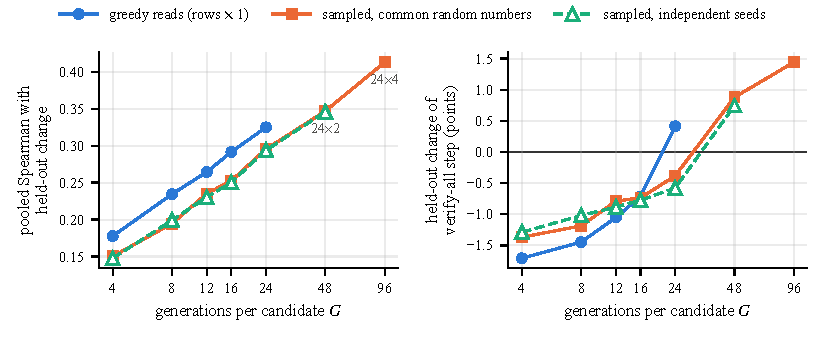
\includegraphics[width=0.85\linewidth]{figures/verify_cost.pdf}
\caption{\textbf{Verification quality is set by the number of fresh generations} (exploratory; 11
pools, 400 random question/sample subsets per cell). $G$: generations per candidate; rows: training
questions; sampled verifiers use one sample per question up to $24$ questions, then $24\times2$ and
$24\times4$. Left: pooled Spearman with the held-out change. Right: held-out change realized by a
verify-all step (ties broken uniformly).}
\label{fig:verify}
\end{figure}

\section{Self-optimization end to end}
\label{sec:experiments}

\subsection{End-to-end structural search}
\label{sec:exp-search}
End to end, task and optimizer model are \greater{}'s Llama-3-8B-Instruct and Gemma-2-9B-it, on its
21 BIG-Bench Hard tasks \citep{suzgun2023bbh} (50 train, 100 dev, up to 100 test questions), GSM8K
\citep{cobbe2021gsm8k} and FOLIO \citep{han2024folio}, split with a fixed seed; $41\%$ of our BBH
test questions were used to produce \greater{}'s published prompts, so comparisons with those prompts
are also reported on the clean remainder. The structural search (Algorithm~\ref{alg:search},
Appendix~\ref{app:search}) runs on Llama-3-8B and seven tasks (six BBH tasks and FOLIO) for $12$
rounds ($K=6$ proposals per slot, shortlist $3$), in arms that differ only in shortlist or
verification: patch-v50 (fixed-reasoning objective) and random-v50 (random shortlist), both verified
on all $50$ training questions, and random-v8 ($8$-question minibatches); textgrad-v50 (textual
gradients) is a different method class with its own proposals. The distributional
arm, registered conditional on H-dist or H-inc, is not run. The registered comparisons, paired by
seed within tasks, are patch-v50 vs.\ random-v50 (does the shortlist signal matter under full verification?) and
random-v50 vs.\ random-v8 (does the verification budget matter?); the prompt selected on dev is
evaluated on test once, with three numerical re-rolls (deterministic engine, $4{,}096$ tokens).
\todo{Seeds 1--3: test accuracy per task
and mean (full, clean); paired differences, conditional and task-level intervals, W/T/L;
textgrad-v50 (seeds 1--2); truncation; GPU time, tokens; the seven tasks.}

\subsection{Does \greater{} need its gradient?}
\label{sec:exp-greater}
The official \greater{} code (Llama-3-8B, our $50$ training questions, $106$ steps, top-$k$ $40$,
top-$q$ $6$, batch $64$; memory-only patches, Appendix~\ref{app:greater}) runs with its gradient
shortlist and with a shortlist drawn uniformly from the same model-proposed candidates, on tasks
fixed in advance because \greater{}'s published prompts gain most there: tracking shuffled objects
(five objects) and geometric shapes. \todo{Gradient vs.\ random shortlist: test accuracy of final
prompts (deterministic engine; full, clean) vs.\ the initial prompt; two registered repetitions per
arm (candidate sampling unseeded); wall time.}

\subsection{Breadth}
\label{sec:exp-breadth}
\todo{Configuration chosen end to end (random-v50 if it matches patch-v50) on 21 BBH tasks, GSM8K
and FOLIO, Llama-3-8B and Gemma-2-9B, vs.\ ZS-CoT and \greater{}'s initial and published prompts;
full and clean subsets; $4{,}096$ tokens; truncation and cost.}
